\documentclass[../sparc.tex]{subfiles}
\graphicspath{{\subfix{../images/}}}
\begin{document}

%%%%%%%%%%%%%%%%%%%%%%%%%%%%%%%%%%%%%%%%%%%%%%%%%%%%%%%%%%%%%%%%%%%%%%%%%%%%%%%%
\section{Басовый ключ}
\index{Музыка!Басовый ключ}

Кроме скрипичного ключа в музыке часто используется \emph{басовый ключ}.  Обычно
басовый ключ используется для тех музыкальных инструментов, у которых частотный
диапазон находится ниже, чем охватывает скрипичный ключ.

Мнемоника для басового ключа представлена на
рис. \ref{fig:lilypond-music-graph-2}.

\begin{figure}[ht]
  \caption{Мнемоника для запоминания нот басового ключа.}
  \begin{tikzpicture}
    \node (image) at (4, 2) {
      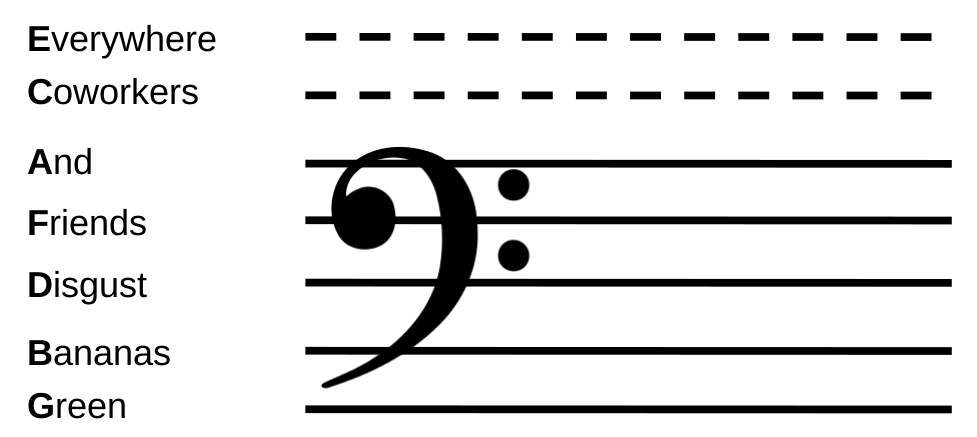
\includegraphics[width=8cm]{music-bass-clef-mnemonic}
    };
    \draw[thick, ->] (0, -1.0) -- (10, -1.0) node[anchor=north east] {x (Время)};
    \draw[thick, ->] (0, -1.0) -- (0, 4.0) node[anchor=north east] {y (Частота)};
  \end{tikzpicture}
  \label{fig:lilypond-music-graph-2}
\end{figure}

\end{document}
